\documentclass[../main.tex]{subfiles}	



\begin{document}
	
\chapter{Healthy-Faulty Signal Classification}

In the second part of this thesis, we will apply the complex-valued deep learning framework, developed in part 1, to a real world problem of condition monitoring in industrial applications.\\
Condition Monitoring is defined as \textit{the process of monitoring a parameter of condition in machinery (vibration, temperature, etc.), in order to identify a significant change which is indicative of a developing fault}.\\
In our technological and industrial society, the use and mastery of condition monitoring turned out to be of extreme importance, since it allows to be schedule maintenance, or other actions to be taken in order to prevent consequential damage and avoid its, often expensive, consequences. Furthermore, it can helps in increasing the lifespan of many engines, preventing faults that could develop in major failures.\\	
Condition Monitoring techniques are normally used on rotating equipment, auxiliary systems and other dynamic machinery (compressors, pumps, electric motors, etc.) while for static devices, usually, periodic inspections are sufficient.\\
In our analysis, we will propose a modification (or, better, an extension) to the existing approach to the strategy that is usually followed for rotating machines, i.e. \textbf{vibration analysis}.\\

What engineers do, is usually taking measurements on machine bearing casings with \textit{accelerometers} to measure the casing vibrations, sometimes provided also of electric transducers able to directly observe the rotating shafts and detect their radial (and axial) displacements. Data collected are then set of vibrational signals that can be analyzed and studied to detect clues of something bad that is happening. Vibration levels can then be compared with some historical baseline values (a "ground truth") derived after long periods of experiments, and in some cases compared with established standards such as load changes, to keep high the attention. Vibration limits can also be defined based on the machine design or components, knowing their fault frequencies of bearings.\\
Interpreting the vibration signal obtained is an elaborate procedure that requires specialized training and experience. With the technology progresses and increasingly complicated machines, simple comparisons and vibration limits are not anymore sufficient to guarantee the performances and accuracies needed by the companies. Luckily, also the techniques available have widely improved: thanks especially to the recent advances of machine and deep learning, signal analysis and classification is strongly simplified. Several state-of-the-art approaches have been developed, able to provide the vast majority of data analysis automatically, retrieving information instead of raw data.\\
In general one commonly employed technique is to examine the individual frequencies present in the signal. These frequencies, in fact, can correspond to certain mechanical components or specific malfunctions (e.g. unbalance or misalignment). So, by analyzing these frequencies and their harmonics, a specialist can in principle be able to identify the location or the type of a problem, sometimes even the cause. And this is possible weeks, even months, before the effective failure or damage of the apparatus, giving ample time to the technicians for replacing or repairing the machine. \\
But the interesting part in this approach is that we have a mathematical instrument that allow us to move from the time to the frequency domain, with all the consequent advantages: the \textbf{Fourier Transform}. We will see, in the next section, that this operator not only permits the analysis of the frequency spectrum of the signal, but also represents the connection among the real-valued measurements of physical quantities and the complex-valued domain in which we can effectively put to test the framework we have developed.\\
It is however better to specify that frequency analysis tends to be most useful on machines that employ rolling element bearings and whose main failure modes tend to be the degradation of those bearings, which typically exhibit an increase in characteristic frequencies associated with its geometries and constructions.\\
Tons of different "manual" analysis are possible for those kind of signals in the frequency domain, a study of its phase spectrum for example, but in this thesis we are not really interested in them since we will rely on modern deep learning approaches, providing also efficient alternatives to the actual state-of-the-art techniques.


\section{State-of-the-Art}

In chapter \ref{}, we were complaining about the fact that literature does not provide almost any kind of complex-valued dataset to effectively test the models we have developed. There, we were forced to "manually construct" our data, with simple distributions of points satisfying certain properties \ref{}, or clever modifications of existing real collections \ref{}. Relying on them could have been fine for that preliminary analysis, mainly focused on the convergence and the stability of the training process, rather then on the final performances. However, we believe that, in order to prove the efficacy of our method, we should stress our complex-valued architectures on more concrete and reliable datasets.\\
But, is there the possibility of measuring in some way physical quantities that are inherently complex-valued? From this point of view, the answer is yes, and we just need to think about magnetic momenta. The PHD thesis we have based our work on \ref{}, is constructed exactly on these kind of data: Magnetic Resonance Images contains, in fact, much information in their phase, that, with a complex neural network the author managed to outperform many existing approaches that used to discard such information.\\
But we should not limit our horizons when we have a powerful instrument like the Fourier transform $\mathcal{F}$, that allow us to associate a complex-valued frequency domain representation to a function of time. In this new representation, the magnitude represents the amount of a certain frequency present in the original signal, while the argument is its phase offset with respect to the basic sinusoid. All of this means that, given any dataset composed of waves in the time domain, the same can be studied in the frequency domain exploiting the new power of complex-valued models, keeping all the physical information without need of expedients like before. Several papers have been published, suggesting complex-valued models to study electric, seismic \ref{} and vibrational signals in the complex domain. So, in principle, for any signal registered in the time domain, we can recover, and maybe exploit, the phase information thanks exactly to the Fourier transform.\\
Studying the problem in the frequency domain is a quite common approach to signal processing, since many operations in the time domain have a complex counterpart that sometimes turns out to be easier to perform (eg. differentiation and convolution). Furthermore, also from a purely theoretical point of view, several concepts are easier to derive and understand with complex notations.

\subsection{Baseline Machine Learning}

But how can we effectively distinguish among vibration signals? According to the traditional machine learning approach we should rely on some hand-crafted features extractable from the wave in the time domain; those features can then face a dimensionality reduction step (PCA, t-SNE, etc.) and then sent through baseline classifiers like Support Vector Machines or Multi-Layer Perceptrons. This was the fundamental strategy for years: in term of memory and time complexity it is very efficient, because each sample is reduced to a handful of meaningful values, but, in general, it lacks of generalization capabilities, since the high-level features to be used are chosen every time by an expert, depending on the situation, and also from the point of view of the accuracy reached, more modern technologies employing deep learning are already able to outperform it.

\subsection{Study in the frequency domain}

However, even if condition monitoring is not one of the main tasks over which machine learning researchers focused mostly in the last years, several techniques and improvements could be recovered and re-adapted from the popular area of audio applications. In the end, in fact, sounds are vibrations of the air, and so their analysis can present interesting similarities with our problem.\\
It is exactly from the widely developed theory of deep learning applied to audio processing, that we inherit techniques suitable to study a wave signal in the frequency domain. The computational instrument that allow us to do so is the \textbf{Short-Time Fourier Transform} (\textbf{STFT}). Discrete STFT is a method of partitioning
continuous signals (in the time-dependent representation) over a long period into shorter segments (usually overlapped) at short time intervals, and
applying a Fourier transform to each of those segments. An additional step can be taken, at this point, deriving the power spectrum of the signal: taking the square modulus of the STFT we can construct a 2D sample, i.e. an image, representing the amplitude of the signal for a particular frequency at a particular time.\\
In figure \ref{fig:example_stft} we took a random signal from the dataset we are going to study, and we applied the STFT: the leftmost picture represents the original wave, the central one is the result after the application of the transform (so the signal in the frequency domain), while the rightmost is its power spectrum. 
\begin{figure}[!ht]
	\centering
	\includegraphics[scale=0.5]{example-image-b}
	\caption{Example signal}
	\label{fig:example_stft}	
\end{figure}
After the computation of the power spectrum for each vibration signal at this point, there are two directions that the researcher can decide to follow:
\begin{itemize}
	\item keeping the two-dimensional input and building a machine learning classifier able to work directly with the spectrograms (usually a Convolutional Neural Network);
	% ADD SOURCE
	\item taking a further step and extracting from the spectrogram the so called \textit{Mel Frequency Cepstral Coefficients} (MFCC): these coefficients, widely used in speech recognition tasks, permit an efficient compression of the "important information" carried by the signal, and can be simply given in input to an ordinary classifier.
\end{itemize}
Even if they were not properly designed for vibration analysis applied to condition monitoring, the usage of MFCCs can bring very good results together with an high efficiency in term of space and time complexity, because of the information compressed.\\
In figure \ref{fig:summary_hf_classification_methods} are represented schematically the two main state-of-the-art approaches (high-level features extraction vs power spectrograms) for healthy-faulty vibration signal classification, that we just described.\\
\begin{figure}[!ht]
	\centering
	\includegraphics[width=\textwidth]{pictures/summary_hf_classification_methods.pdf}
	\caption{State-of-the-art approaches for vibration data classification applied to predictive maintenance (source: \cite{deep_learning_vibration_gravity}).}
	\label{fig:summary_hf_classification_methods}	
\end{figure}
In the successive analysis, we will propose an alternative to the approaches listed above, that is more suitable to complex-valued deep learning: the coefficients of a Fourier transform are, in fact, inherently complex, and so, instead of losing all the phase information taking the power spectrum (that is constituted only by their amplitudes), we stop one step before keeping the original complex-valued variables. In the end, deriving the complex spectrum is equivalent to computing a discrete Fourier transform over short overlapping windows of the signal.

\section{Bonfiglioli}

The main motivation of this thesis work was the development and testing of an unconventional deep learning approach, based on complex-valued neural networks, on a series of datasets provided to FBK by Bonfiglioli \ref{fig:bonfiglioli_logo}, a worldwide designer, manufacturer and distributor of a complete range of gearmotors, drive systems, planetary gearboxes and inverters.\\
\begin{wrapfigure}{r}{0.5\textwidth}
	\includegraphics[width=0.5\textwidth]{pictures/bonfiglioli_logo.pdf}
	\caption{Bonfiglioli logo.}
	\label{fig:bonfiglioli_logo}
\end{wrapfigure}
The company provided a large number of datasets collected from as many experiments, with the purpose of simulating artificially the most frequent faults, that usually occur over the bearings of different kind of engines.


\subsection{Simulation Environment}

Data have been collected at the Bonfiglioli headquarters of Rovereto (TN), with the experimental setup schematized in figure \ref{fig:bonfiglioli_experimental_setup}.
\begin{figure}[!ht]
	\centering
	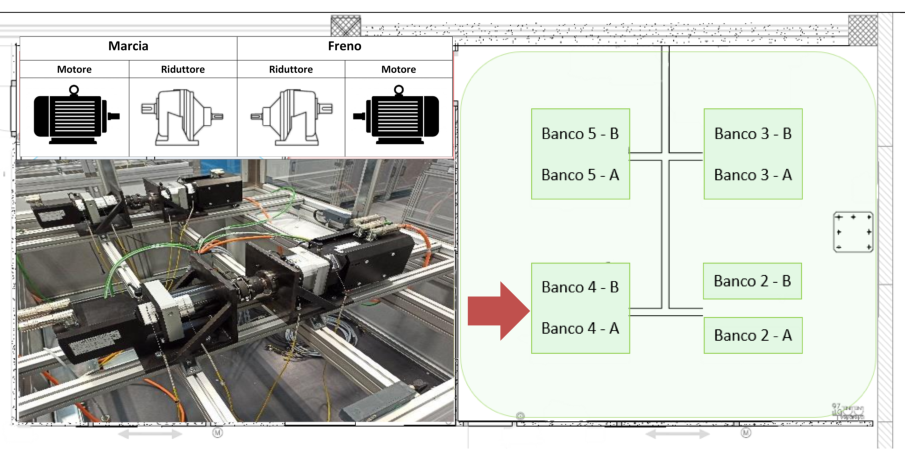
\includegraphics[width=\textwidth]{pictures/bonfiglioli_experimental_setup}
	\caption{Schematic representation of the experimental workbench used by Bonfiglioli.}
	\label{fig:bonfiglioli_experimental_setup}	
\end{figure}
The laboratory is constituted of four different workbenches in which different experiments can be conduced. In each workbench, a lab-scale rotating simulation equipment is installed, constituted 

In the experiments, faults were artificially simulated using mechanical tricks (e.g. unbalance is simulated attaching a small object to the shaft)

data were collected through an accelerometer fixed over the bearing
+ other measurements

% explain periodic working cycle of 120h


\subsection{Datasets}

In these last months, the Bonfiglioli laboratory have setup different experiments, in order to provide data relative to different kind of engines and for different types of simulated faults. For each of those runs, containing 120 hours of measurements, a dataset in \texttt{.h5} format has been provided, with the values registered during a working cycle. Those datasets had an internal structure quite mazy, and so we had to rely on a custom library, provided by FBK researchers, to load and process the data. Each sample contains several entries, related to the different variables measured during the process: beyond vibration signals collected through the accelerometers, Bonfiglioli decided to monitor also the temperature of some components, voltage and current flowing through them, together with the phase information of the inverter. Additionally, for the experiments realized more recently, they used an additional component in their setup, a \textit{multiplier}, providing a second vibration signal.\\
However, for what concern our work, we are interested only in vibration signals.


In table \ref{} we leave a small summary containing the main technical details relative to each trial that we decided to use in our analysis. 

Another interesting fact to specify is that 


Sampling was performed
because a vibration is a periodic signal in the time domain [43], and most fault signals have
periodicity. Therefore, sampling is used to examine the consistency and continuity of each
condition using the features calculated from the signals

The signal segmentation for sampling was based on the rotational frequency of the
rotor. Generally, in rotating equipment, the rotational frequency is the most dominant
component, and the majority of fault components appear in the harmonic form of the
rotational frequency.

Then describe train-test split and number of signals of each type



\subsection{Baseline Classification Approach}




\section{Mendelay Data}

The last dataset we are going to analyze for this chapter is the Mendeley Dataset \cite{mendeley_dataset}: a collection of vibration signals collected from bearings with different health conditions and under different time-varying speed conditions. The problem is again an healthy-faulty classification task with two different "bad" classes: faulty with an inner race defect and faulty with an outer race defect. \\
The experiments have been realized over a machinery fault simulator with the setup shown in \ref{fig:mendeley_setup}. 
\begin{figure}[!ht]
	\centering
	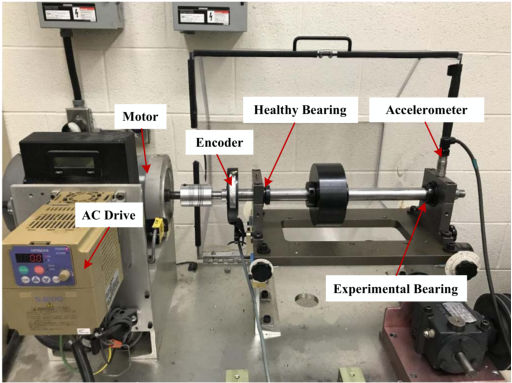
\includegraphics[width=0.5\textwidth]{pictures/mendeley_setup.pdf}
	\caption{Experimental setup for Mendeley data.}
	\label{fig:mendeley_setup}
\end{figure}
The shafts is driven by a motor which rotational speed is controlled by an AC Drive. Two ball bearings are installed to support the shaft: the left one is healthy, while the one on the right is the experimental bearing, replaced during each experiment with a component of a different health condition. Again, vibration data are collected thanks to an accelerometer fixed on the housing of the experimental bearings,  while an incremental encoder is used to collect the rotational speed values.\\
These datasets were collected and reorganized with the purpose of evaluating the effectiveness of methods developed for bearing fault diagnosis under time varying speed conditions. This last point is the main difference with most of vibration datasets available from actual literature, that have been collected under constant speed condition (as Bonfiglioli's). The complex-valued models we have developed so far, however, were not properly designed to work on such dynamic signals, but this still represents an opportunity to stress and push to the limit the approach we have designed.

\subsection{Dataset Structure}

Given the various general purposes for which this dataset was designed (i.e. condition monitoring and analysis of bearings' frequency characteristics under time-varying rotational speed conditions), its internal structure is slightly intricate. First of all, each sample has two channels, one for vibration data and the other for rotational speed data. Each signal is sampled at 200000 Hz and the sampling duration is 10 s. There whole collection of signals is divided into 36 different datasets, depending on two experimental settings:
\begin{itemize}
	\item \textit{health condition} (healthy, faulty with inner race defect, faulty with outer race defect);
	\item \textit{speed varying condition} (increasing speed, decreasing speed, increasing then decreasing speed and decreasing then increasing speed).
\end{itemize} 
Therefore, there are 12 different cases for configuration, each of them constituted of 3 trials, to ensure the authenticity of the data, that explain the 36 subsets.




	
\end{document}